
\begin{frame}{Result 1 - Background - \WhileCC\ Programming Language}
    \pause
    \footnotesize
    \begin{minipage}[t]{0.33\linewidth}
        \vspace{0.05em}
       \center
        \textbf{\color{Blue}{Syntax}
        }
         \begin{itemize}
                \vspace{0.5em}
                \pause \item Terms
                \vspace{-0.5em}
                        \begin{align*}
                         t^s ::= x^s\ \mid F(t_1^{s_1}, \ldots , t_m^{s_m})
                        \end{align*}
                \vspace{-2.7em}
                \pause \item Statements
                \vspace{-0.5em}
                    \begin{align*}
                        &S ::=\\
                                &\ \mathsf{skip}\
                                \mid \mathsf{div}
                                \mid \bar{x} := \bar{t}
                                \mid S_1\ S_2\\
                                &\mid \mathsf{if}\ b \ \mathsf{then}\ S_1 \ \mathsf{else}\ S_2\ \mathsf{fi}\ \\
                                &\mid \mathsf{while}\ b\ \mathsf{do}\ S_0\ \mathsf{od}
                                \\
                                &\mid n:= \textcolor{BrickRed}{\mathsf{choose\ }} (z: \nat): P(z,\bar{t})
                    \end{align*}
                \vspace{-1.7em}
                \pause \item Procedures
                    \begin{center}
                        $P$ ::= $\mathsf{proc} \ D\ \mathsf{begin}\ S\ \mathsf{end}$
                    \end{center}
                        
            \end{itemize}
    \end{minipage}
    \begin{minipage}[t]{0.34\linewidth}
         \pause 
         \begin{center}
            \vspace{0.2em}
             \textbf{\color{Blue}Algebra $\algebraR$}
         \end{center}
         \begin{center}
            \fbox{
            \begin{tabular}{ll}
                 & $\realZero$, $\realOne$, $\realMinusOne$ : $\ \totalTo \mathbb{R}$ \\
                  & $\realPlus$, $\realTimes$ : $\Reals\times\Reals\totalTo\Reals$\\
                  & $\natPlus$, $\natTimes$ : $\Nats\times\Nats\totalTo\Nats$\\
                  & {\color{BrickRed} $\realInv$ : $\Reals\ \to\ \Reals$} \\
                  & $\natZero$ : $\ \totalTo \Nats$ \\
                  & $\natSuc$ : $\Nats\totalTo\Nats$ \\
                  & $\true$, $\false$ : $\ \totalTo\Bools$ \\ 
                  & $\boolAnd$, $\boolOr$ : $\Bools\times\Bools\totalTo\Bools$ \\
                  & $\boolNot$ : $\Bools\totalTo\Bools$ \\
                  & $\natEq$, $\natLess$ : $\Nats\times\Nats\totalTo\Bools$ \\
                  & {\color{BrickRed} $\mathsf{=_{real}}$, $\realLess$ : $\Reals\times\Reals \ \to\ \Bools$} 
            \end{tabular}    
            }
        \end{center}
        
    \end{minipage}
    \begin{minipage}[t]{0.30\linewidth}
        \pause
        \begin{center}
             \vspace{0.2em}
             \textbf{\color{Blue}{Semantics} }
         \end{center}            
            \begin{align*}
            \realInv(x) = &
                \begin{cases*}
                    1/x & if $x \neq 0$\\
                    {\color{BrickRed}\uparrow} & {\color{BrickRed}otherwise}
                \end{cases*}\\
            \mathsf{=_{real}}(x,y) = &
                \begin{cases*}
                    \false\ & if $x \neq y$\\
                    {\color{BrickRed} \uparrow\ }& {\color{BrickRed} otherwise}
                \end{cases*}\\
            \realLess(x,y) = &
                \begin{cases*}
                    \true\ & if $x<y$\\
                    \false\ & if $x>y$\\
                    {\color{BrickRed}\uparrow} & {\color{BrickRed} if $x=y$}\\
                \end{cases*}
            \end{align*}
        \setlength{\fboxsep}{0pt}
        \fbox{
        \begin{tabular}{l}
            The Semantics of a program $P$\\
            is denoted by a many-valued\\
        function $P^\algebraR$.
        \end{tabular}
        }
    \end{minipage}
    \note[itemize]{
    The functions commonly known as inverse, equality and order are not continuous.
    Since the concepts of \While{}-computability and \WhileCC-computability
    We are using here have been designed to make all expressed functions continuous on their domains \citep{ComputableFunctionsAndSemicomputableSetsOnManySortedAlgebras-TuckerAndZucker_Handbook_2001, AbstractVSConcreteComputationOnMetricPartialAlgebras_TuckerZucker_2004},
    the discontinuities in conventional models of equality, order, and inverse
    have been resolved by making the functions in $\mathcal{R}$ undefined there.
    }
        
\end{frame}


\begin{frame}{Result 1 - Background}
    \pause
    \begin{definition}[\WhileCC-approximability, \citep{ModelOfCompForPartFunc_MingQuanFuAndJeffZucker}]
\label{def::whileCC-approximable}
    A \WhileCC-procedure $P$ of type $\real\times\nat \to \real$ on $\algebraR$ is said to \textit{approximate} a function $f:\Reals\to\Reals$ iff for all $n\in \Nats$ and all $x\in \Reals$:
    \begin{itemize}
        \pause \item $x \in \dom(f) \then \emptyset \neq P^\algebraR(x,n) $ \pause  $\subseteq \Nbd(f(x), 2^{-n})$
            , and
        \pause \item $x \notin \dom(f) \then P^\algebraR(x)=\emptyset$
    \end{itemize}
    \pause where $\Nbd(y,r)$ has the standard definition of neighborhood on $\Reals$ i.e., \[\Nbd(y,r) = \{ z\in \Reals\ \mid \abs{y-z}<r \}.\]
\end{definition}

     \begin{exampleblock}{\textbf{\textcolor{OliveGreen}{Goal}}}
         Construct \WhileCC-procedures approximating elementary functions by induction
     \end{exampleblock}
     
     \begin{exampleblock}{\textcolor{BrickRed}{\textbf{Challenge:} Using comparison operators introduces undefinedness.}}
        \pause How do we \WhileCC-approximate ``piecewise'' functions?
     \end{exampleblock}

    \note[itemize]{Let us start with a more formal definition. We already defined the \WhileCC programming language earlier, but what does it mean for a function to be \WhileCC-approximable?\\
    The semantics for \WhileCC-programs is a multi-valued function. Now let's say $P$ is a \WhileCC-procedure with a real and a precision variable in \Nats as inputs. It is said to approximate a function $f$ on the reals if for any input in the domain of $f$, it gives us a nonempty set of values all close enough to $f(x)$. The definition of closeness (here, neighborhood) is the standard definition of neighborhood on the reals. }
\end{frame}

\begin{frame}{Result 1 - Challenges}
    \begin{minipage}[t]{0.4\linewidth}
        \vspace{-2em}
        \begin{exampleblock}{\color{BrickRed}\textbf{Problem}}
            When defining piecewise functions, comparison makes a hole! 
        \end{exampleblock}
        \pause
        \vspace{0.75em}
        {\textbf{\color{MidnightBlue}Example: Even Root} \pause \textbf{\color{BrickRed} - First Attempt}\\}
        \footnotesize
        \vspace{-1em}
        \[ 
            \BLOCK{
            \PROC  \\
                \INDENT{
                \IN\ x:\real\ c:\nat}\\
            \BEGIN \\
                \INDENT{
                \IF x \realLess 0 \THEN \\
                    \INDENT{
                    \RETURN 0}\\
                \ELSE \\
                    \INDENT{
                    \RETURN \mathsf{Root}(x,c)}\\
                \FI \\

                }\\
            \END}\\
        \] 
        \pause
        \begin{flushright}
        % \includegraphics[width=.98\linewidth]{root.png}
            \vspace{-3em}
            \pause
            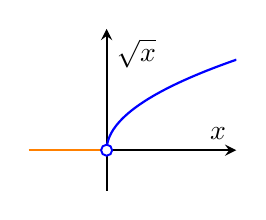
\begin{tikzpicture}
    \begin{axis}[
        width = 120,
        axis lines=middle,
        xlabel=$x$, ylabel=$\sqrt{x}$,
        samples=200,
        domain=-3:5,
        ymin=-1, ymax=3,
        xmin=-3, xmax=5,
        grid=both,
        thick, 
        xtick =\empty,
        ytick=\empty
    ]
    
    % Plot f(x) = 0 for x < 0
    \addplot[orange, thick, domain=-3:0] {0};
    
    % Plot f(x) = sqrt(x) for x > 0
    \addplot[blue, thick, domain=0:5] {sqrt(x)};
    
    % Open circle at (0,0) to indicate undefined
       \fill[color=white,draw=blue,line width=0.7pt] (axis cs:0,0) circle (2pt);
    
    \end{axis}
\end{tikzpicture}

        \end{flushright}
    \end{minipage}
    \begin{minipage}[t]{0.50\linewidth}
      
              
    \end{minipage}

\end{frame}


\begin{frame}{Result 1 - Challenges}
    \begin{minipage}[t]{0.4\linewidth}
        \vspace{-2em}
        \begin{exampleblock}{\color{BrickRed}\textbf{Problem}}
            When defining piecewise functions, comparison makes a hole! 
        \end{exampleblock}
        \pause
        \vspace{0.75em}
         \begin{exampleblock}{\textbf{Solution}}
            \begin{itemize}
                \pause \item Find an overlapping interval where both pieces are defined
                \pause \item Use the nondeterminism of ``choose''  
            \end{itemize}
            % Assuming we have $\isCloseEnough(q,c,n) \implies \abs{\sqrt[c]{q}} < 2^{-n}$ 
            \pause
                       
        \end{exampleblock}     

        \pause
    \end{minipage}
    \begin{minipage}[t]{0.50\linewidth}
        % \vspace{-2em}
        \pause
        {
        \vspace{-1.5em}
        \center
        }
        \vspace{-1em}
        \scriptsize
         \[ 
            \BLOCK{             
                \PROC  \\
                    \INDENT{
                    \IN \ x:\real\ c:\nat \\
                    \AUX \chosenVal:\nat\ l:\real}\\
                \BEGIN \\
                    \INDENT{
                    l := \CHOOSE (q:\real) :
                                        \BLOCK{
                                        \isCloseEnough(q, c, n)} \\
                     \\
                    \chosenVal := \CHOOSE (k : \nat) :
                            \BLOCK{
                            \PROC \\
                                \INDENT{
                                \IN k:\nat\ x:\real}\\
                            \BEGIN \\
                                \INDENT{
                                \IF k \natEq 1 \THEN \\
                                    \INDENT{
                                    \RETURN 0<x}\\
                                \ELSE \IF k \natEq 2 \THEN \\
                                    \INDENT{
                                    \RETURN x<l}\\
                                \ELSE \\
                                    \INDENT{
                                    \RETURN \false}\\
                                \FI }\\
                            \END}\\
                    \IF \chosenVal \natEq 1 \THEN \\
                        \INDENT{
                        \RETURN \mathsf{Root}(x,c)}\\
                    \ELSE \IF \chosenVal \natEq 2 \THEN \\
                        \INDENT{
                        \RETURN 0}\\
                    \FI}\\
                \END}\\
            \] 
        \pause
        \begin{flushright}
        % \includegraphics[width=.98\linewidth]{root.png}
            \vspace{-8.5em}
            \pause
            
\begin{tikzpicture}
  \begin{axis}[
    width=\linewidth,
    axis lines=middle,
    xlabel=$x$, ylabel=$y$,
    xmin=-10, xmax=24,      % show x>0 up to 24
    ymin=-4.5, ymax=8,
    domain=0:24, samples=300,
    xtick =\empty, 
    ytick =\empty, 
  ]
    \addplot[name path=upperpink, thick] {sqrt(x) + 2};
    \addplot[name path=lowerpink, thick] {sqrt(x) - 2};
    
    \addplot[gray, domain=-10:24] {0};
    \addplot[blue, thick, domain=-10:0] {0}node[pos=0.92, below left] {$y=0$};
    

    \addplot[dashed, red, thick] coordinates {(4,-4.5) (4,8)};
    
    \addplot[fill=pink!50, draw=none] fill between[of=upperpink and lowerpink];
    \addplot[blue, very thick] {sqrt(x)}node[pos=0.80, above] {$y=\sqrt{x}$};
    
    \addplot[only marks, mark=*, mark size=3pt, blue] coordinates {(0,0)};
    \draw[->, thick, cyan] (axis cs:4,-3) -- (axis cs:-10,-3) node[above right] {compute y = 0};
    \fill[color=white,draw=cyan,line width=0.7pt] (axis cs:4,-3) circle (3pt);
    
    \draw[->, thick, magenta] (axis cs:0,-3.8) -- (axis cs:24,-3.8) node[above left] {approximate $\sqrt{x}$};
    \fill[color=white,draw=magenta,line width=0.7pt] (axis cs:0,-3.8) circle (3pt);

  \end{axis}
\end{tikzpicture}

        \end{flushright}
        
    \end{minipage}

\end{frame}